\documentclass[11pt, a4paper]{article}

\usepackage[english,francais]{babel}
\usepackage[utf8]{inputenc}
\usepackage[T1]{fontenc}
\usepackage[pdftex]{graphicx}
\usepackage{setspace}
\usepackage[french]{varioref}
\usepackage{amsfonts}
\usepackage{amssymb}
\usepackage{geometry}
\usepackage{amsthm}
\usepackage[french, ruled]{algorithm2e}
\geometry{margin=2cm}

\usepackage{tikz}
\usetikzlibrary{calc}   % coordinate calculation
\usepackage{xifthen}

\title{Rassemblement d'agents mobiles}
\author{\'Eloi Perdereau}
%\date{}

\newcommand{\spacee}[2] {
  \begin{tikzpicture}[thick, scale=0.6]
    \def \step {1}
    \def \cc {\step/2}  % center of cell
    \coordinate (offset) at ($(\cc,\cc)$);
    \draw[step=\step] (0,0) grid ($#1$);   % draw the grid, base at #1
    % draw the neighbors
    \foreach \coord in #2 {
      \coordinate[at=\coord, name=A];
      \draw ($(A) + (offset)$) circle ({\cc*0.8});
    }
  \end{tikzpicture}
}

\newcommand{\case}[2] {
  \begin{tikzpicture}[thick, scale=0.6]
    \def \step {1}
    \def \cc {\step/2}  % center of cell
    \coordinate (offset) at ($(\cc,\cc)$);
    \draw[step=\step] (0,0) grid ($(3,3)$);   % draw the grid, base at #1
    % draw the center circle
    \draw ($(1,1) + (offset)$) circle (\cc*0.8);
    % draw the neighbors
    \foreach \coord in #1 {
      \coordinate[at=\coord, name=A];
      \draw ($(A) + (offset)$) circle ({\cc*0.8});
    }
    % draw the movement arrow if #3 is not empty
    \ifthenelse{\equal{#2}{}}{}{
    \draw[->] ($(1,1) + (offset)$) -- ($#2 + (offset)$);
    }
  \end{tikzpicture}
}

\theoremstyle{plain}
\newtheorem{thm}{Theorem}[section]
\newtheorem{lem}[thm]{Lemma}
\newtheorem{prop}[thm]{Proposition}
\newtheorem*{cor}{Corollary}

\theoremstyle{definition}
\newtheorem{defn}{Definition}[section]
\newtheorem{conj}{Conjecture}[section]
\newtheorem{exmp}{Example}[section]

\theoremstyle{remark}
\newtheorem*{rem}{Remark}
\newtheorem*{note}{Note}

\begin{document}

\maketitle

\section{Cas}

On omet les cas symétriques par rapport au robot du milieu
(rotations de $90^{\circ}$, $180^{\circ}$ et $270^{\circ}$.)

\subsection{0 ou 1 voisins}
\case {{}}                        {}
\case {{(0,0)}}                   {(0,0)}
\case {{(1,0)}}                   {(1,0)}
\case {{(2,0)}}                   {(2,0)}

\subsection{2 voisins}
\case {{(0,0),(1,0)}}             {(1,0)}
\case {{(0,0),(2,0)}}             {(1,0)}
\case {{(2,0),(1,0)}}             {(1,0)}
\case {{(0,0),(2,1)}}             {(1,0)}
\case {{(2,0),(0,1)}}             {(1,0)}
\case {{(0,1),(1,0)}}             {(0,0)} \\

\case {{(0,2),(2,0)}}             {}
\case {{(0,1),(2,1)}}             {}

\subsection{3 voisins}
\case {{(0,0),(1,0),(2,0)}}       {(1,0)}
\case {{(2,0),(1,0),(2,1)}}       {(1,0)}
\case {{(0,0),(1,0),(2,1)}}       {(1,0)}
\case {{(2,0),(1,0),(0,1)}}       {(1,0)}
\case {{(0,0),(2,1),(2,2)}}       {(1,0)}
\case {{(2,0),(0,1),(0,2)}}       {(1,0)} \\

\case {{(0,0),(2,1),(2,0)}}       {(1,0)}
\case {{(0,0),(0,1),(2,0)}}       {(1,0)} \\

\case {{(0,0),(0,1),(2,1)}}       {}
\case {{(0,2),(2,2),(2,0)}}       {}
\case {{(0,2),(2,2),(1,0)}}       {}
\case {{(1,0),(0,1),(2,1)}}       {}
\case {{(1,2),(0,1),(2,0)}}       {}

\subsection{4 voisins}
\case {{(0,0),(1,0),(2,0),(2,1)}} {(1,0)}
\case {{(0,0),(1,0),(2,0),(0,1)}} {(1,0)} \\

\case {{(0,0),(1,0),(2,0),(2,2)}} {}
\case {{(0,0),(1,0),(2,0),(1,2)}} {}
\case {{(0,2),(1,2),(2,1),(2,0)}} {}
\case {{(0,2),(1,2),(2,1),(1,0)}} {}
\case {{(0,2),(1,2),(2,1),(0,0)}} {}
\case {{(0,0),(1,0),(2,1),(0,1)}} {} \\

\case {{(0,2),(1,2),(2,0),(1,0)}} {}
\case {{(0,2),(1,2),(2,0),(0,0)}} {}
\case {{(0,2),(1,2),(2,0),(0,1)}} {}
\case {{(0,2),(1,2),(1,0),(0,0)}} {}
\case {{(0,2),(2,2),(2,0),(0,0)}} {}
\case {{(1,2),(2,1),(1,0),(0,1)}} {}


\subsection{5 voisins et plus}
Pour énumérer les cas avec 5 et 6 robots voisins, il suffit de prendre le
complémentaire des cas avec respectivement 3 et 2 robots voisins.
Aucun de ces cas n'entraine un mouvement de la part du robot concerné.

\subsection{Extension}

Tel quels, les cas 6 et 13 peuvent conduire à une déconnexion de l'espace. Pour
y remédier, il faut que chaque robot mémorise son entourage d'une ronde sur
l'autre (il ne retient que son entourage précédent.) Puis, si à la ronde
précédente, il était dans le cas 6 ou 13, il faut qu'il vérifie si au moins une
des cases suivante contient un robot : à droite, en bas et en bas à droite. Si
ce n'est pas le cas, il revient à sa position précédente. Les cas symétriques
sont définis de façon analogues. \\

Après avoir réglé ces cas de déconnexions, un autre problème survient avec les
cas 5 et 6. Il se peut que l'espace alterne entre deux états ce qui rend le
rassemblement impossible. Le problème vient du fait que des robots disposés en
quinconce soient de nouveau en quinconce à la ronde suivante (avec des
positions inversés.) Et ainsi, revenir à la position qu'ils occupaient deux
rondes plus tôt.  Pour y remédier, on va de nouveau utiliser l'entourage de
la ronde précédente : Si à la ronde précédente, un robot était dans le cas 5 ou
6, et qu'il est désormais dans le cas opposé, alors il ne bouge pas pour cette
ronde. \\

\subsection{Formalisation}
\begin{algorithm}[H]
  $finish \leftarrow False$\;
  $k \leftarrow 0$\;
  \While{not $finish$} {
    $N_k \leftarrow get\_neighbors()$\;
    \uIf{$k \% 4 = 0$} {
      % test d'arrêt
      \uIf{$N_k$ is case $1.1.1$ or \\
          ($N_k$ is case $1.1.\{2,3,4\}$ and $N_{k-2}=rotate180(N_k)$) or \\
          ($N_k$ is case $1.3.2$         and $N_{k-2}=rotate90 (N_k)$) } {
          $finish \leftarrow True$\;
      }
      % mouvement si il n'y a personne en (i,j-2) ou (i+1,j-2)
      \ElseIf{$(i, j-2)$ and $(i+1, j-2)$ are both empty or both full} {
        move according to $N_k$\;
      }
    }
    \Else{
      \If{($N_{k-1}$ is case $1.2.\{4,5\}$ or $1.3.\{5,6\}$) and
          ($(i,j+1)$, $(i-1,j)$, $(i-1,j+1)$ are all empty)} {
          move to $(i-1,j)$\;
      }
    }
    $k \leftarrow k+1$\;
  }
  \caption{}
\end{algorithm}

\newcommand{\Gathered}{\ensuremath{\textsc{gathered}}\xspace}

\section{A single robot on the topmost row}

We denote by $r(t)$ the single robot in the topmost row of the bounding box at
step $t$. If there are more than one robot in the topmost row, $r(t)$ is not
defined.  The row and column of the cell occupied by $r(t)$ would be denoted
$Y(t)$ and $X(t)$ respectively. In general we will assume $Y(t)=0$ unless
otherwise stated.  The global configuration of robots at time $t$ would be
denoted by $C(t)$. If $C(t)$ satisfies the terminating conditions of the
algorithm then it is called a \Gathered configuration.

\begin{prop}
If $r(t)$ exists and is on $(0,i)$, then there was a robot on cell $(0,i-1)$,
$(0,i)$ or $(0,i+1)$ (or on cell $(-1,i-1)$, $(-1,i)$ or $(-1,i+1)$) at step
$t-1$.
\end{prop}

\begin{prop}
At step $t$, if a robot $w$ was not in the neighborhood of $r(t)$, then robot
$w$ cannot be on the topmost row in step $(t+1)$.
\end{prop}

The above properties imply that studying the neighborhood of $r(t)$ for new
robots on the topmost row is sufficient to determine if the topmost row moved
down.

\begin{lem}
If $r(t)$ exists and the current configuration $C(t)$ is not  \Gathered then
there exists a constant $c$ such that after $c$ steps, either $BB(t+c) \subset
BB(t)$ (i.e. the topmost row moves down) or a \Gathered configuration is
reached.
\end{lem}

\begin{proof}

We define the graph $G_{single}(V_{single}, E_{single})$ as follows :
\begin{itemize}
  \item $V_{single}$ : neighborhood cases of $r(t)$
  \item $(u,v) \in E_{single}$ if $u$ is the neighborhood of $r(t)$ and $v$ is
        the neighborhood of $r(t+1)$ such that $Y(t)=Y(t+1)$ and the
        configuration $C(t+1)$ is not \Gathered.  \end{itemize}
The graph generated by considering all possible single step transformations is
shown on figure \ref{graph:single}. If a node has no outgoing edges then in the
next step $(t+1)$ either there are no robots on row $Y(t)$ or a \Gathered
configuration is reached. So the sink nodes in the graph satisfy the lemma.  We
notice multiple cycles in the graph; if any cyclic path is followed by the
algorithm then the topmost row might never move down. However, edges of the
graph only represent single step transformations. We will show that the cyclic
paths are not followed by the algorithm by studying 3 paths in the graph and
this would be sufficient to prove that the lemma holds. \\
%i.e. $BB(t+c) \subset BB(t)$. \\

\noindent
We denote by $A$ to $G$ the 7 nodes of $G_{single}$ from top to
bottom and left to right. \\ A transformation corresponding to an edge in
$G_{single}$ is called a \emph{Left-move}, \emph{Mid-move}, or
\emph{Right-move}, if  $X(t) > X(t+1)$, $X(t) = X(t+1)$, or $X(t) < X(t+1)$
respectively.\\
Let $t$ be the step at which the algorithm reaches the first node of the
considered path, i.e. the neighborhood of $r(t)$ is represented by this node.
For each path, the first edge is a \emph{Right-move}. \\
Every neighborhood requirements stated below have been programmatically tested.

%The middle robot in the start node is at $(0,0)$ at $t$.
\begin{enumerate}

% \item Consider the path ($D \rightarrow A \rightarrow B$).
%       Let $t$ be the step at which the algorithm reaches node $D$, i.e. the
%       neighborhood of $r(t)$ is represented by $D$. According to the rule
%       (1.2.1), the robot $r(t)$ would move down. So if the algorithm follows
%       edge $D \rightarrow A$, then some other robot must move up to row $Y(t)$.
%       The only possibility is the robot at ($Y(t)+1,X(t)$) to move up to
%       ($Y(t),X(t)-1$) using rule (1.2.6). This implies that in step $t$, the
%       row $Y(t)+2$ was empty at columns $X(t)+1$ to $X(t)-1$. Moreover, in step
%       $(t+1)$, row $Y(t+1)$ is empty at $X(t+1)+1$ and $X(t+1)+2$. So if node
%       $A$ is not a \Gathered configuration, then there must be a robot
%       neighboring the right bottom corner of node $A$. The only possibility is
%       the cell $Y(t+1)+2, X(t+1)$ to be occupied in step $t+1$.  Thus in the
%       next step, the topmost row will move down. So, the path ($D \rightarrow A
%       \rightarrow B$) cannot exist in any execution of the algorithm.

\item Consider the path ($B \rightarrow C \rightarrow D$).
      For the algorithm to follow edge $B \rightarrow C$, one of the following
      neighborhood is required : \\
      \spacee {(5,4)} {{(1,2),(1,1),(2,1),(3,0)}}
      \spacee {(5,4)} {{(1,2),(1,1),(2,1),(3,0),(4,0),(4,1)}} \\
      According to the rule (1.3.5), the robot at ($X(t)+1,Y(t)+1$) will move
      down and occupy ($X(t+1),Y(t+1)+2$). \\
      Yet, for the algorithm to follow edge $A \rightarrow B$ at (t+1), the
      cell ($X(t+1),Y(t+1)+2$) must be empty. \\
      Thus, the path ($B \rightarrow C \rightarrow D$) cannot exist in any
      execution of the algorithm.
      Analogously, the path ($D \rightarrow A \rightarrow B$) cannot exist
      either.

% \item Consider the path ($D \rightarrow B \rightarrow C$).
%       Let $t$ be the step at which the algorithm reaches node $D$, i.e. the
%       neighborhood of $r(t)$ is represented by $D$.
%       By enumerating every possibility for $r(t)$ to follow edge $D \rightarrow
%       A$ we see that ($X(t)-2,Y(t)+1$) is empty and the row $Y(t)+2$ is
%       occupied at column $X(t)-2$ and empty at columns $X(t)+1$ to $X(t)-1$.
%       Thus, according to the rule (1.3.5), the robot at ($X(t)-1,Y(t)+1$) will
%       move down and occupy ($X(t+1),Y(t+1)+2$). Moreover, for the algorithm to
%       follow edge $A \rightarrow B$, the row $Y(t+1)+2$ must be empty at
%       columns $X(t+1)-1$ to $X(t+1)+1$. So, the path ($D \rightarrow A
%       \rightarrow B$) cannot exist in any execution of the algorithm.

% \item Consider the path ($B \rightarrow E \rightarrow D$).
%       By enumerating every possibility for $r(t)$ to follow edge $B \rightarrow
%       E$ we see that the row $Y(t)+1$ is empty at column $X(t)+2$ and occupied
%       at $X(t)+3$, and the row $Y(t)+2$ is empty at columns $X(t)-1$ to
%       $X(t)+1$ and occupied at $X(t)+2$ and $X(t)+3$.
%       Thus, according to the rule (1.3.6), the robot at ($X(t)+1,Y(t)+1$) will
%       move down and occupy ($X(t+1),Y(t+1)+2$). Moreover, for the algorithm to
%       follow edge $E \rightarrow D$, the row $Y(t+1)+2$ must be empty at
%       columns $X(t+1)-1$ to $X(t+1)+1$. So, the path ($D \rightarrow A
%       \rightarrow B$) cannot exist in any execution of the algorithm.
%       Analogously, the path ($D \rightarrow E \rightarrow B$) cannot exist
%       either.

\item Consider the path ($B \rightarrow E \rightarrow D$).
      For the algorithm to follow edge $B \rightarrow
      E$ we see that the following neighborhood is required : \\
      \spacee {(5,4)} {{(1,2),(1,1),(2,1),(3,0),(4,0),(4,1)}} \\
      According to the rule (1.3.6), the robot at ($X(t)+1,Y(t)+1$) will move
      down and occupy ($X(t+1),Y(t+1)+2$). \\
      Yet, for the algorithm to follow edge $E \rightarrow D$ at (t+1), the
      cell ($X(t+1),Y(t+1)+2$) must be empty. \\
      Thus, the path ($B \rightarrow E \rightarrow D$) cannot exist in any
      execution of the algorithm.
      Analogously, the path ($D \rightarrow E \rightarrow B$) cannot exist
      either ; neither does the paths ($B \rightarrow E \rightarrow B$) and
      ($D \rightarrow E \rightarrow D$) due to the symmetry of the nodes $B$
      and $D$.

\item Consider the path ($B \rightarrow D \rightarrow B$).
      For the algorithm to follow edge $B \rightarrow
      D$ we see that different required neighborhood may occur :
      \begin{itemize}
      \item \spacee {(6,4)} {{(1,2),(1,1),(2,1),(3,1),(4,0),(5,0),(5,1)}}
            \spacee {(6,4)} {{(1,2),(1,1),(2,1),(3,1),(4,0)}} \\
            According to rule (1.2.5), the robot at ($X(t)+2,Y(t)+1$) will move
            down and occupy ($X(t+1)+1,Y(t+1)+2$).
      \item \spacee {(4,4)} {{(1,2),(1,1),(2,1),(3,0)}} \\
            The robot ($X(t)+2,Y(t)+2$) will either not move or move at
            ($X(t+1)+1,Y(t+1)+1$), ($X(t+1),Y(t+1)+2$), or ($X(t+1),Y(t+1)+1$).
            In the latter case, a \Gathered configuration is reached at
            ($t+2$).
      \item \spacee {(4,4)} {{(1,2),(1,1),(2,1),(3,1),(3,0)}} \\
            The robot at ($X(t)+2,Y(t)+1$) will either not move or move at
            ($X(t+1)+1,Y(t+1)+2$) or ($X(t+1),Y(t+1)+2$).
      \item \spacee {(6,4)} {{(1,2),(1,1),(2,1),(3,1)}} \\
            A \Gathered configuration is reached at ($t+2$).
      \end{itemize}
      Yet, for the algorithm to follow edge $D \rightarrow B$ at (t+1), the
      following neighborhood is required \\
      \spacee {(3,4)} {{(1,2),(1,1),(0,1)}} \\
      Thus, the path ($B \rightarrow D \rightarrow B$) cannot exist in any
      execution of the algorithm.
      Analogously, the path ($D \rightarrow B \rightarrow D$) cannot exist
      either.

\end{enumerate}
Due to the above arguments, all cyclic paths can be removed from the graph
$G_{single}$. This directly implies that the statement of the lemma holds.
\end{proof}

The results of this section show that if there is only one robot in topmost
(or bottom-most) row or equivalently if there is only one robot in leftmost (or
rightmost)  column, then the bounding box shrinks within a constant number of
steps.

\section{Multiple robots on the topmost row}

We denote by $l(t)$ the leftmost robot in the topmost row of the bounding box at
step $t$. The row and column of the cell occupied by $l(t)$ would be denoted
similarly to $r(t)$ defined in the previous section.

\begin{prop}
The robot $l(t)$ cannot successively perform \emph{Mid-move}s indefinitely.
\end{prop}

\begin{proof}

We define the graph $G_{leftmost\_mid}(V_{leftmost\_mid},
E_{leftmost\_mid})$ as follows :
\begin{itemize}
  \item $V_{leftmost\_mid}$ : neighborhood cases of $l(t)$.
  \item $(u,v) \in E_{leftmost\_mid}$ if $u$ is the neighborhood of $l(t)$ and
        $v$ is the neighborhood of $l(t+1)$ such that $X(t)=X(t+1)$ and
        $Y(t)=Y(t+1)$ and the configuration $C(t+1)$ is not \Gathered.
\end{itemize}
We notice multiple cycles in the graph; if any cyclic path is followed by the
algorithm then the leftmost robot in the topmost row might never move. However,
edges of the
graph only represent single step transformations. We will show that the cyclic
paths are not followed by the algorithm by studying 3 paths in the graph and
this would be sufficient to prove that the proposition holds. \\

TODO (c'est ok sur papier)

\end{proof}

\begin{prop}
The robot $l(t)$ cannot successively perform a \emph{Left-move}s and a
\emph{Mid-Move} by passing through neighborhoods of (1.3.7), (1.2.2) and
(1.2.3).
\end{prop}

\begin{proof}

We define the graph $G_{leftmost\_left}(V_{leftmost\_left},
E_{leftmost\_left})$ similarly to $G_{leftmost\_mid}$ with $X(t)=X(t+1)-1$. We
will examine it's edges and show that after each of them, a \emph{Mid-move} is
impossible.

\noindent
We denote by $A$ to $H$ the 8 nodes of $G_{leftmost\_left}$ from top to
bottom and left to right. \\

% Let $t$ be the step at which the algorithm reaches the first node of the
% considered path, i.e. the neighborhood of $r(t)$ is represented by this node.
% For each path, the first edge is a \emph{Right-move}. \\
% Every neighborhood requirements stated below have been programmatically tested.

\begin{enumerate}
\item Each destination of edges $(A,B)$, $(A,D)$, $(C,E)$, $(D,E)$, $(D,G)$ and
      $(D,H)$ are sink nodes in $G_{leftmost\_mid}$.

\item For the algorithm to follow the edge $(D,F)$, the following neighborhood
      is required : \\
      \spacee {(5,4)} {{(0,0),(0,1),(1,0),(2,1),(3,1),(3,2)}}
      According to the rule (1.3.5), the robot at ($X(t)-1,Y(t)+1$) will move
      down and occupy ($X(t+1),Y(t+1)+2$). \\
      Yet, for $l(t)$ to perform a \emph{Mid-move} when it's neighborhood is
      node $F$, one of the robots $(X(t)-1,Y(t)+1)$ or $(X(t)+1,Y(t)+1)$ must
      have the neighborhood of rule (1.1.2).
\end{enumerate}

\end{proof}


\appendix

\section{Single robot movements}
\begin{figure}[H]
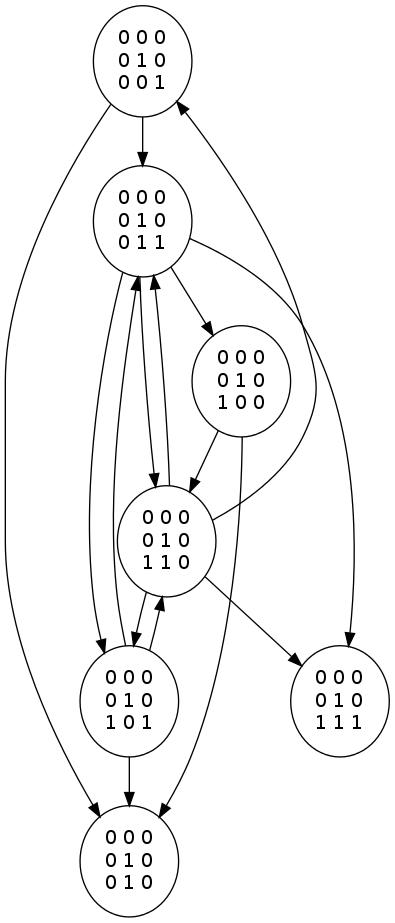
\includegraphics[scale=0.50]{graph_images/graph_single_all.jpg}
\caption{Single robot}
\label{graph:single}
\end{figure}

\section{Leftmost robot \emph{Mid-move}s}
\begin{figure}[H]
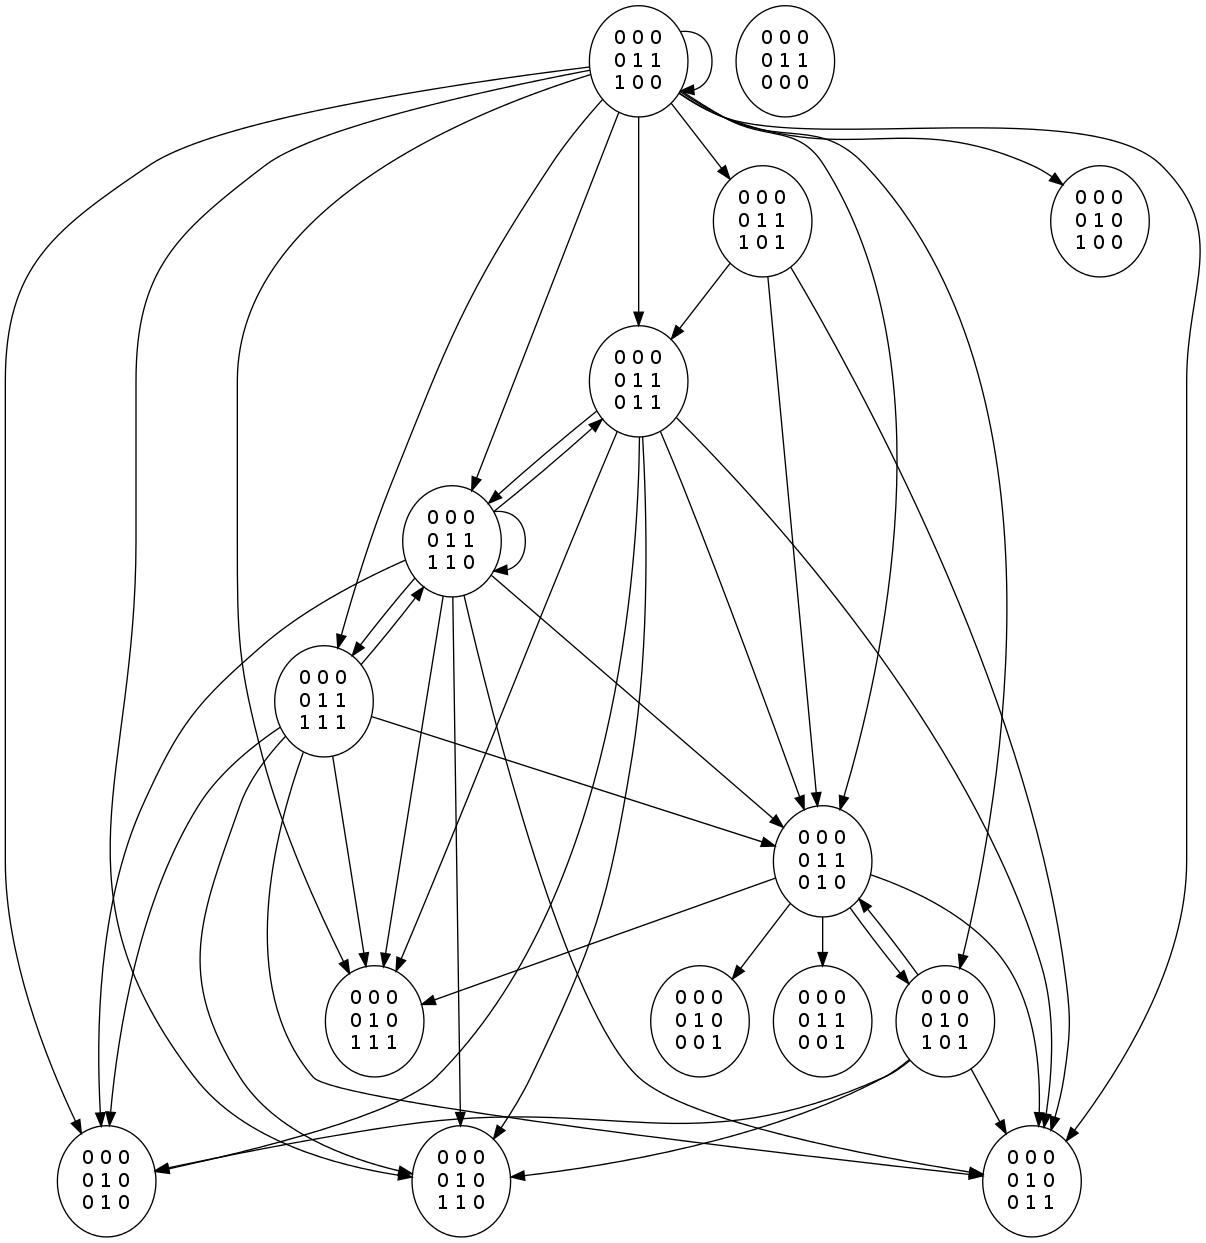
\includegraphics[scale=0.40]{graph_images/graph_leftmost_mid.jpg}
\caption{\emph{Mid-move}}
\label{graph:leftmost_mid}
\end{figure}

\section{Leftmost robot \emph{Left-move}s}
\begin{figure}[H]
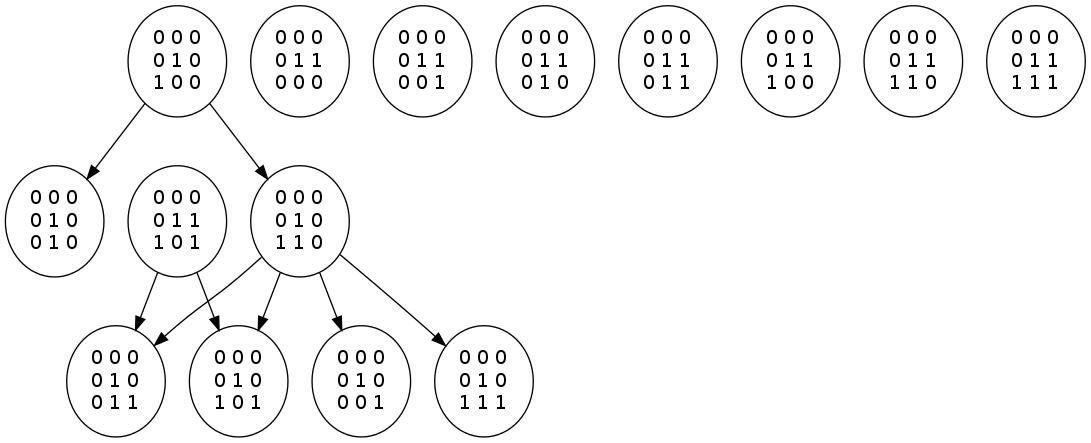
\includegraphics[scale=0.50]{graph_images/graph_leftmost_left.jpg}
\caption{\emph{Left-move}}
\label{graph:leftmost_left}
\end{figure}

\section{Leftmost robot \emph{Right-move}s}
\begin{figure}[H]
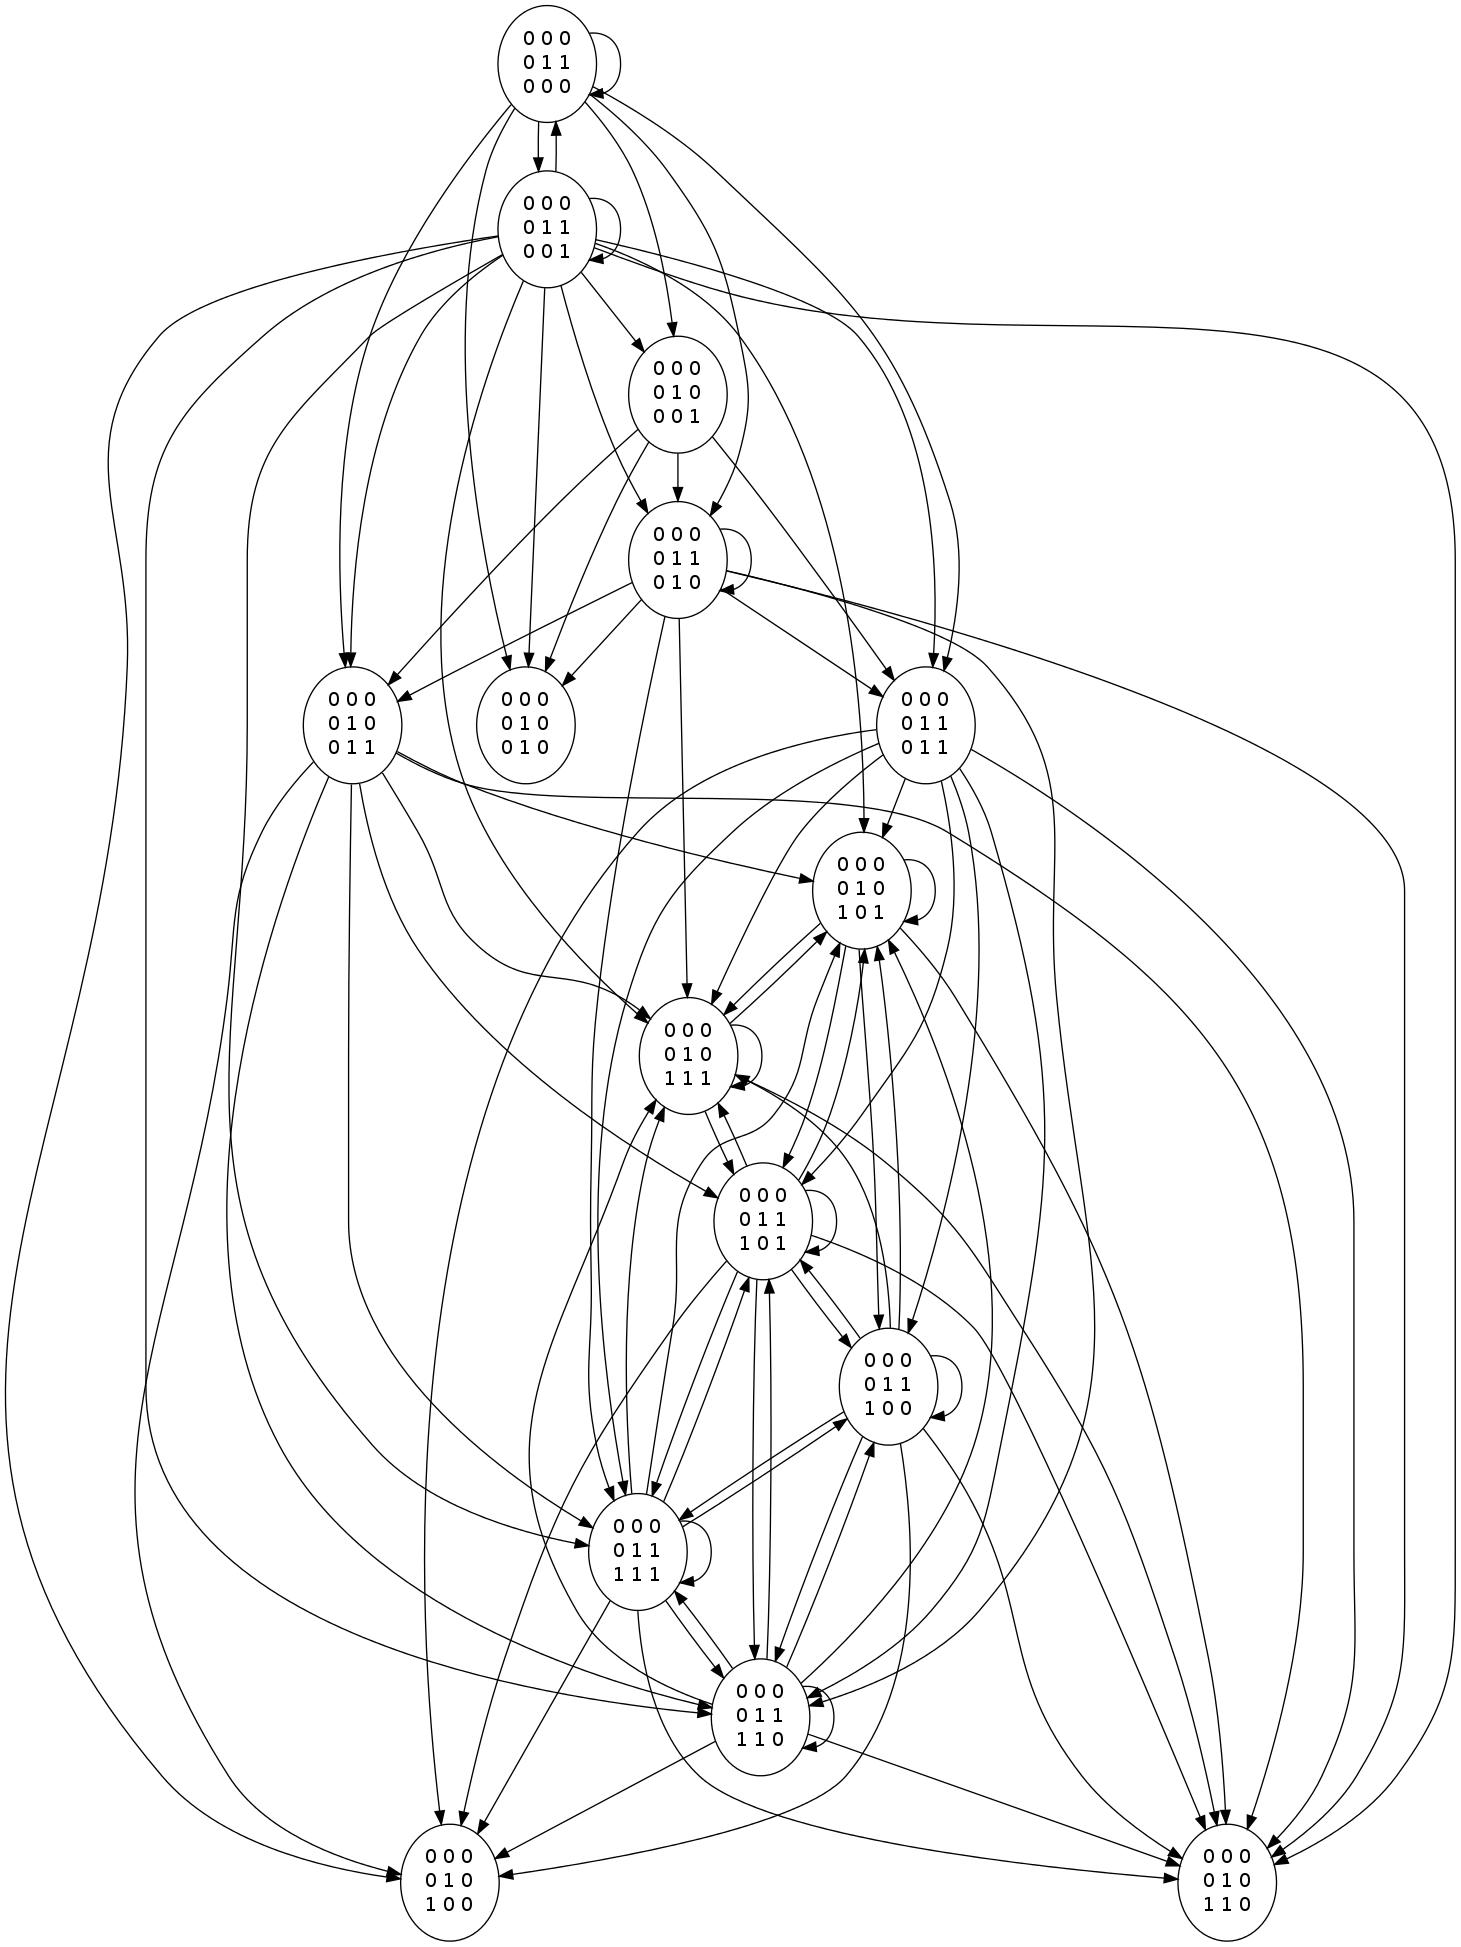
\includegraphics[scale=0.40]{graph_images/graph_leftmost_right.jpg}
\caption{\emph{Right-move}}
\label{graph:leftmost_right}
\end{figure}

\end{document}
